\documentclass[dvipdfmx]{beamer}
\usepackage{mySld}

\begin{document}
\title[OS]{オペレーティングシステム\\第2章 前提知識}
\date{}

\begin{frame}
  \titlepage
\end{frame}

%\begin{frame}
%  \frametitle
%  \tableofcontents
%\end{frame}

\section{コンピュータのハードウェア構成}
\begin{frame}
  \frametitle{ハードウェア構成}
  \fig{scale=0.41}{hardBlock-crop.pdf}
  \begin{itemize}
    \item SMP(Symmetric Multiprocessing)
    \item CPU,メモリ,タイマー,アダプタ,コントローラ,バス
    \item DMA(Direct Memory Access),I/O完了割込み
  \end{itemize}
\end{frame}

\section{CPUの構成}
\begin{frame}
  \frametitle{CPUの構成}
  \fig{scale=0.5}{cpuBlock-crop.pdf}
  \begin{itemize}
    \item PSW(Program Status Word)
    \item CPUレジスタ
    \item 割り込み(Interrupt)
  \end{itemize}
\end{frame}

\section{最近のコンピュータの実際の構成}
\begin{frame}
  \frametitle{デスクトップ・パーソナルコンピュータ}
  \fig{scale=0.5}{intelDesktop-crop.pdf}
  \begin{itemize}
    \item CPU
    \item コア(Core)
  \end{itemize}
\end{frame}

\begin{frame}
  \frametitle{サーバコンピュータ}
  \fig{scale=0.4}{intelServer-crop.pdf}
\end{frame}

\section{オペレーティングシステムの構造}
\begin{frame}
  \frametitle{オペレーティングシステムの構造}
  \fig{scale=0.49}{osOrganization-crop.pdf}
\end{frame}

\begin{frame}
  \frametitle{プロセスの構造}
  \fig{scale=0.5}{procOrganization-crop.pdf}
\end{frame}

\section{カーネルの構成方式}
\begin{frame}
  \frametitle{単層カーネル(モノリシック・カーネル)}
  \fig{scale=0.49}{osOrganization-crop.pdf}
\end{frame}

\begin{frame}
  \frametitle{マイクロカーネル(micro-kernel)}
  \fig{scale=0.5}{microkernel-crop.pdf}
\end{frame}

\section{TaC}
\begin{frame}
  \frametitle{TaC7とTaC}
  \begin{minipage}{0.58\columnwidth}
    \begin{center}
      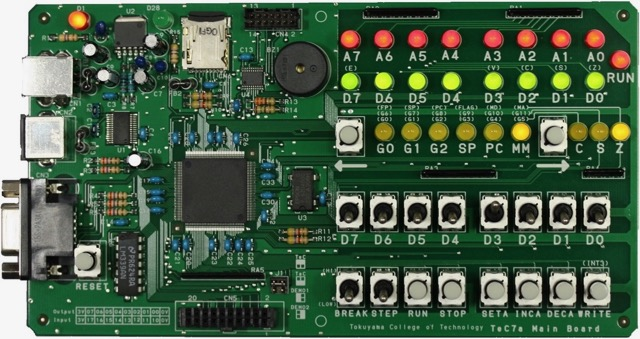
\includegraphics[scale=0.27]{Photo/TeC7.jpg}\\
      (a) TeC7の写真
    \end{center}
  \end{minipage}
  \begin{minipage}{0.38\columnwidth}
    \begin{center}
      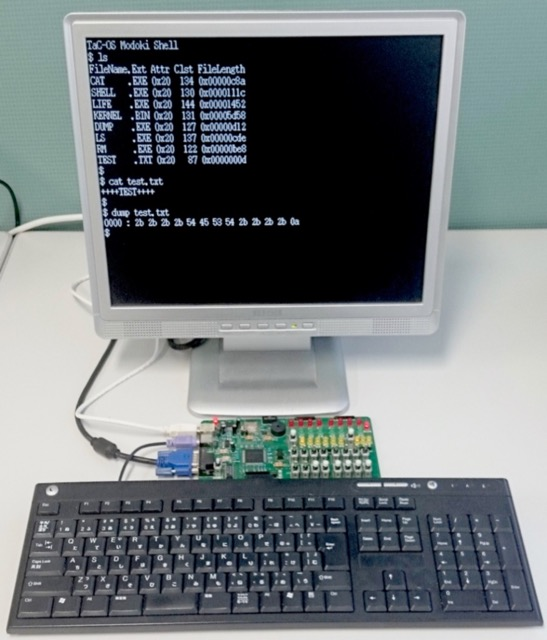
\includegraphics[scale=0.22]{Photo/TaC.jpg}\\
      (b) TaCとしての使用例
    \end{center}
  \end{minipage}
\vfill
TeC7は,TacOSを書き込んだマイクロSDカードを装着すると,
簡単なPC(TaC)として使用できる.
\end{frame}

\begin{frame}
  \frametitle{TaCのハードウェア}
  \fig{scale=0.49}{tacBlock-crop.pdf}
\end{frame}

\begin{frame}
  \frametitle{TacOSの構造}
  \fig{scale=0.49}{tacosOrganization-crop.pdf}
\end{frame}

\section{もう一つの仮想マシン}
\begin{frame}
  \frametitle{Type 2 ハイパーバイザ}
  \fig{scale=0.6}{type2Hypervisor-crop.pdf}
  \begin{itemize}
  \item ホスト・オペレーティングシステム
  \item ゲスト・オペレーティングシステム
  \item VMware Workstation, VirtualBox
  \end{itemize}
\end{frame}

\begin{frame}
  \frametitle{Type 1 ハイパーバイザ}
  \fig{scale=0.6}{type1Hypervisor-crop.pdf}
  \begin{itemize}
  \item メインフレーム: IBM z/VM
  \item PCサーバ: VMware vSphere, Xen, Hyper-V
  \end{itemize}
\end{frame}

\begin{frame}
  \frametitle{仮想アプライアンス}
  \begin{itemize}
  \item 仮想マシンのディスクイメージの配布
  \item ソフトウェアの新しい流通手法
  \end{itemize}
\end{frame}
\end{document}
